\documentclass[10pt]{article}
\usepackage[margin=0.78in]{geometry}
\usepackage[T1]{fontenc}
\usepackage{lmodern,amsmath,amssymb,booktabs,graphicx,microtype,fancyhdr,longtable}
\usepackage[hidelinks]{hyperref}
\usepackage{xurl}
\pagestyle{fancy}\fancyhf{}\setlength{\headheight}{14pt}
\fancyhead[L]{\small HPS Gaussian-Process Resonance Search}
\fancyhead[R]{\small v6.3.2 / 2016 offset transfer}\fancyfoot[C]{\thepage}
\setlength{\parindent}{0pt}\setlength{\parskip}{5pt}
\setlength{\emergencystretch}{2em}\renewcommand{\arraystretch}{1.10}
\newcommand{\Ah}{\widehat A}\newcommand{\sh}{\widehat\sigma}
\newcommand{\CLs}{\mathrm{CL}_{s}}
\hypersetup{pdftitle={HPS-GPR v6.3.2: 2016 offset and response transfer appendix},pdfauthor={Emrys Peets}}
\begin{document}\setcounter{page}{10}
\begin{center}{\LARGE Appendix: offset and response transfer}\\[5pt]
{\large 2016 Gaussian signals at controlled exposure factors 0.1 and 1}\\[4pt]
Emrys Peets\quad---\quad24 September 2026\end{center}


\section*{Question, scope and independent cohorts}

\textbf{No automatic exposure transfer or production correction is justified.} The simple null-offset scaling law is not exact in this conditional experiment. 

Nominal 42 MeV gives $\delta_{100}-10\delta_{10}=+5977$ candidates (pointwise 95\% paired bootstrap interval [3105, 8872]); Stress 76 MeV gives $\delta_{100}-10\delta_{10}=-7279$ candidates (pointwise 95\% paired bootstrap interval [-10911, -3903]). 

Same-source calibration can center held-out toys; transfer to another generator requires separate validation. The offset, signal response and finite-grid limits below are conditional on pinned sources, Gaussian generation/extraction and the archived-kernel GP prescription.

The masses are 42, 44, 60, 66, 76, 90, 92, 117, 160 and 178 MeV. Exposure factors $L=0.1$ and $1$ scale the same full-exposure generating mean. They are paired by Poisson thinning within a cohort and source; nominal and stress cohorts are independent. Toy IDs are shared across masses and injection levels. Counts of fits below therefore do not count independent experiments.

\begin{center}\small\begin{tabular}{llcrr}\toprule
Cohort & Sources & $z$ levels & Backgrounds/cell & Free fits\\\midrule
Pilot & Nominal & 0 & 100 & 2,000\\
Calibration & Nominal, stress & $0,1,\ldots,8$ & 100 & 36,000\\
Evaluation & Nominal, stress & 0, 1, 3, 5 & 100 & 16,000\\
\bottomrule\end{tabular}\end{center}


The saved run contains 2,000/2,000 valid pilot free fits, 36,000/36,000 valid calibration free fits, 16,000/16,000 valid evaluation free fits. Native full-exposure CLs limits are valid for 8,000/8,000 attempts. The failure ledger has 0 rows. Numerical validity is separate from scientific closure.

The nominal pilot defines $s_0(m,L)$, the mean returned Gaussian yield error, independently at each exposure. Signal-bin counts are Poisson with fixed expectation $A=z s_0$ and full-selected Gaussian probabilities. Outside-support loss is retained; training-sideband injection is included; there is no window renormalization. The same expected yield is used for nominal and stress generators. $z$ is a reference-strength label, not a significance.

\subsection*{Why the offset may become more visible}

In a local linear approximation, write the mean background residual as $Lr$ and the effective covariance as $LV$. For a fixed signal vector $w$,\[\delta_L=\frac{w^\top(LV)^{-1}(Lr)}{w^\top(LV)^{-1}w}=L\delta_1,\qquad\sigma_L\simeq\sqrt{L}\sigma_1,\qquad\frac{\delta_L}{\sigma_L}\simeq\sqrt L\frac{\delta_1}{\sigma_1}.\]Thus $\delta_{100}\simeq10\delta_{10}$ and $\bar p_{100}\simeq\sqrt{10}\bar p_{10}$. These are testable approximations, not identities of the count-dependent GP and nonlinear likelihood. Changing the kernel, mask, generator shape or effective covariance invalidates a simple exposure-only transfer.

The existing nine-page 2021 study is preserved unchanged. This appendix is a separate 2016 Gaussian experiment; it does not revise the earlier MC/Gaussian measurements or turn their diagnostics into calibrated limits.

\textbf{Practical interpretation.} One observed 10\% fitted yield or residual is not an ensemble bias: it includes counting noise and possible model mismatch. Transferring it by a factor of ten is not justified by the exposure label alone. A production correction requires qualified background sources, selection-equivalent historical input and independent full-exposure validation, with offset, response and width uncertainties propagated. This appendix changes no production limits.

\clearpage\section*{Exposure scaling of the null offset}


Calibration null fits define $\widehat\delta_L=\overline{\Ah_L(0)}$. The null pull is $p=\Ah/\sh_A$. Because the returned errors fluctuate, the mean pull need not equal $\widehat\delta_L/\overline{\sh_A}$. Exposure differences preserve the nested background pairing.

\begin{center}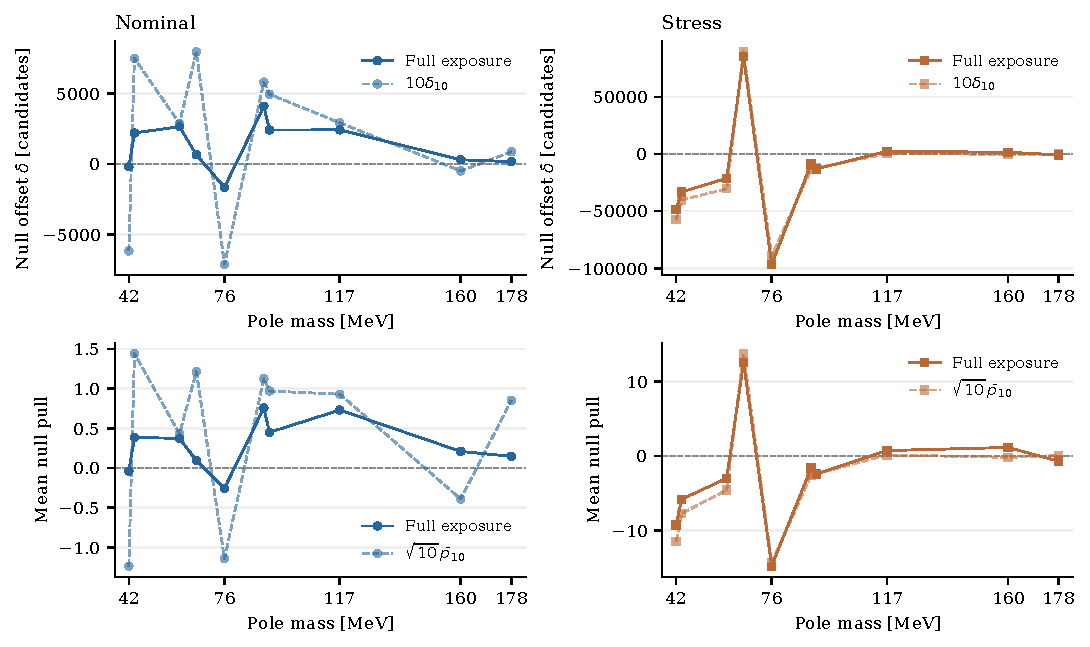
\includegraphics[width=\textwidth]{../figures/exposure_scaling.pdf}\end{center}
{\small Calibration measurements. Solid: full exposure. Dashed: the 10\% estimate transferred using the stated factor. Nominal (blue) and stress (orange) are separate fixed generating means.\par}


\begin{center}\small\begin{tabular}{lrrrr}\toprule
$m$ [MeV] & Nominal $\Delta\delta$ & Nominal $\Delta\bar p$ & Stress $\Delta\delta$ & Stress $\Delta\bar p$\\\midrule
42 & 5976.8 $\pm$ 1466.6 & 1.20 $\pm$ 0.29 & 8866.6 $\pm$ 1452.0 & 2.24 $\pm$ 0.29\\
44 & -5290.3 $\pm$ 1549.9 & -1.06 $\pm$ 0.30 & 7018.0 $\pm$ 1471.6 & 1.89 $\pm$ 0.28\\
60 & -228.2 $\pm$ 1945.0 & -0.06 $\pm$ 0.29 & 9181.9 $\pm$ 1971.9 & 1.57 $\pm$ 0.30\\
66 & -7302.5 $\pm$ 2094.0 & -1.12 $\pm$ 0.32 & -3946.8 $\pm$ 1983.6 & -1.16 $\pm$ 0.30\\
76 & 5468.3 $\pm$ 1692.9 & 0.89 $\pm$ 0.27 & -7279.1 $\pm$ 1795.9 & -0.46 $\pm$ 0.29\\
90 & -1716.3 $\pm$ 1521.5 & -0.37 $\pm$ 0.29 & 4758.1 $\pm$ 1461.6 & 1.00 $\pm$ 0.28\\
92 & -2530.9 $\pm$ 1494.3 & -0.52 $\pm$ 0.29 & -722.3 $\pm$ 1379.9 & -0.02 $\pm$ 0.27\\
117 & -502.9 $\pm$ 818.6 & -0.20 $\pm$ 0.26 & 1919.0 $\pm$ 917.6 & 0.58 $\pm$ 0.29\\
160 & 793.8 $\pm$ 401.3 & 0.60 $\pm$ 0.32 & 1859.9 $\pm$ 372.8 & 1.33 $\pm$ 0.29\\
178 & -700.5 $\pm$ 346.9 & -0.71 $\pm$ 0.34 & -789.6 $\pm$ 310.0 & -0.76 $\pm$ 0.30\\
\bottomrule\end{tabular}\end{center}


{\small $\Delta\delta=\delta_{100}-10\delta_{10}$ (candidates), $\Delta\bar p=\bar p_{100}-\sqrt{10}\bar p_{10}$. Errors are pointwise standard errors; the paired bootstrap intervals are retained in \texttt{scaling\_comparisons.csv}.\par}

\clearpage\section*{Freeze the response before testing the correction}


At each source, exposure and mass, the independent calibration cohort fixes\[\widehat\delta=\overline{\Ah(0)},\qquad\widehat R=\frac{\overline{\Ah(3s_0)-\Ah(0)}}{3s_0},\qquad\widetilde A=\frac{\Ah-\widehat\delta}{\widehat R}.\]The $z=3$ definition is fixed in advance. Held-out $z=1,3,5$ paired responses test its transfer across strength. A constant offset cancels exactly from paired response; subtracting it cannot restore a response slope below one.

\begin{center}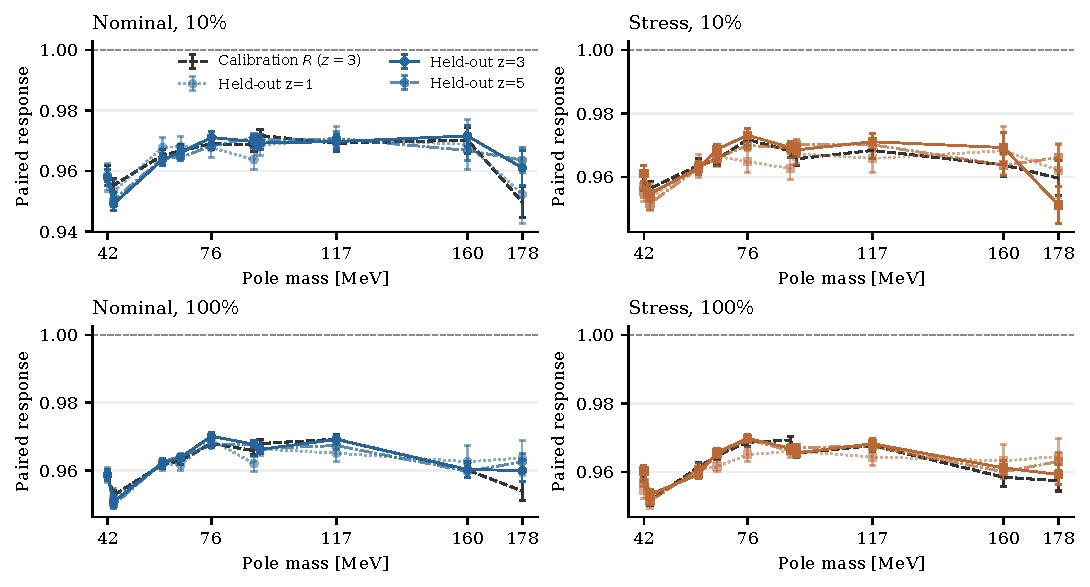
\includegraphics[width=\textwidth]{../figures/response_transfer.pdf}\end{center}
{\small Frozen calibration $R$ (black dashed, standard-error bars) and held-out raw paired responses at three positive injection levels. Bars summarize toy variation; the independent calibration table is not refitted using evaluation toys.\par}


\begin{center}\small\begin{tabular}{lrrrrr}\toprule
Source & Exposure & Frozen $R$ & $z=1$ & $z=3$ & $z=5$\\\midrule
Nominal & 10\% & 0.950--0.972 & 0.952--0.971 & 0.949--0.972 & 0.950--0.971\\
Nominal & 100\% & 0.953--0.969 & 0.952--0.969 & 0.951--0.970 & 0.950--0.968\\
Stress & 10\% & 0.956--0.972 & 0.954--0.968 & 0.951--0.973 & 0.952--0.970\\
Stress & 100\% & 0.952--0.969 & 0.952--0.966 & 0.953--0.970 & 0.952--0.970\\
\bottomrule\end{tabular}\end{center}


{\small Ranges span the ten correlated mass cells; they are not pooled estimates. Full cell values, complete-pair counts and uncertainty are in the CSV tables.\par}

\begin{center}\footnotesize\begin{tabular}{lrrrrr}\toprule
Source & $z$ & Raw & Transfer offset & Direct offset & Affine\\\midrule
Nominal & 0 & [-0.48, 0.85] & [-1.06, 1.16] & [-0.22, 0.09] & [-0.22, 0.09]\\
Nominal & 3 & [-0.57, 0.75] & [-1.17, 1.04] & [-0.31, -0.01] & [-0.22, 0.10]\\
Stress & 0 & [-14.52, 12.52] & [-0.86, 1.59] & [-0.21, 0.25] & [-0.21, 0.25]\\
Stress & 3 & [-14.60, 12.41] & [-0.95, 1.47] & [-0.30, 0.16] & [-0.21, 0.25]\\
\bottomrule\end{tabular}\end{center}


{\small Full-exposure mean-pull ranges across mass cells, using each source's own frozen calibration. Brackets also denote ranges, not confidence intervals.\par}

The offset-transfer diagnostic uses $10\widehat\delta_{10}$ at full exposure; direct-offset subtraction uses the full-exposure calibration offset. The affine diagnostic also divides by the corresponding calibrated response. None of these corrected estimators is inserted into the native profile likelihood or used to rescale a published upper limit.

\clearpage\section*{Held-out pulls after the frozen correction}


For positive $\widehat R$, the statistical-only corrected error and pull are\[\sh_{\widetilde A}=\sh_A/\widehat R,\qquad p_{\rm affine}=\frac{\Ah-\widehat\delta-\widehat R A}{\sh_A}.\]These treat the calibration table as frozen. Its offset/response covariance is retained separately for approximate propagated uncertainty. The calibration null scale $k_0=\operatorname{SD}[(\Ah(0)-\widehat\delta)/\sh_A]$ is also saved; dividing by it is a separate diagnostic, not part of the primary pull.

\begin{center}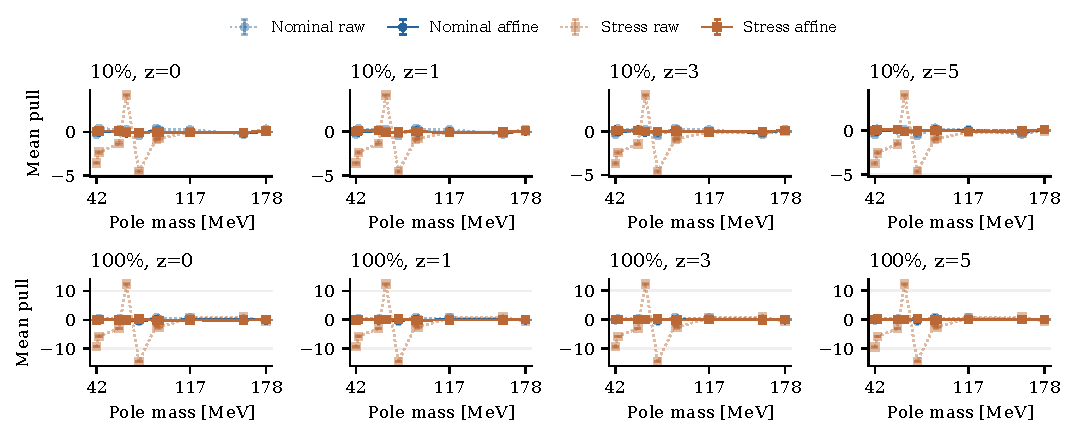
\includegraphics[width=\textwidth]{../figures/corrected_pull_means.pdf}\end{center}
{\small Mean raw pulls (dotted, faint) and frozen affine-corrected pulls (solid). Blue: nominal; orange: stress. Bars are standard errors. Each source uses its own calibration.\par}


\begin{center}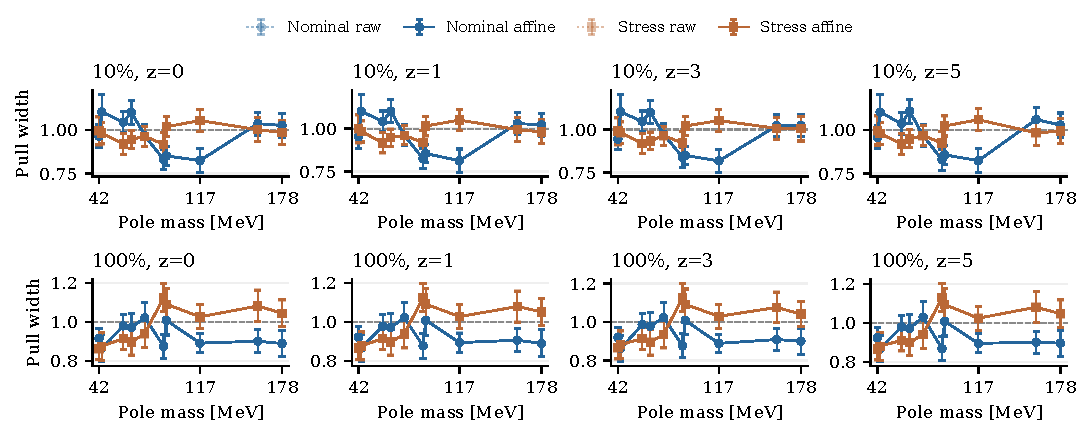
\includegraphics[width=\textwidth]{../figures/corrected_pull_widths.pdf}\end{center}
{\small Corresponding sample pull widths. Bars are bootstrap standard errors. Zero mean and unit width are reference values; successful fits are not selected for agreement with them.\par}


\textbf{Calibration transfer across generators.} Nominal calibration is additionally applied to independent stress toys at full exposure. This is a misspecification check, distinct from each generator's own conditional closure. 

At $z=3$, transferred affine pull means span [-14.25, 12.43] and widths span 0.86--1.13. 

Centering one pinned generator is therefore insufficient evidence that the unknown physical background has been corrected.

\clearpage\section*{A finite-rank Neyman construction}


At each fixed grid value $A=z s_0$, $z=0,\ldots,8$, use the raw signed fitted yield $T=\Ah$ as an ordering statistic. For 100 valid calibration toys, the lower-tail rank probability of a new spectrum is\[p_A(T)=\frac{1+\#\{j:T^{\rm cal}_{A,j}\leq T\}}{101}.\]Reject that grid value when $p_A\leq0.10$. Exchangeability gives rejection probability at most $10/101$ marginally over calibration and evaluation, with conservative ties. This is not a guarantee conditional on the one frozen calibration table.

\begin{center}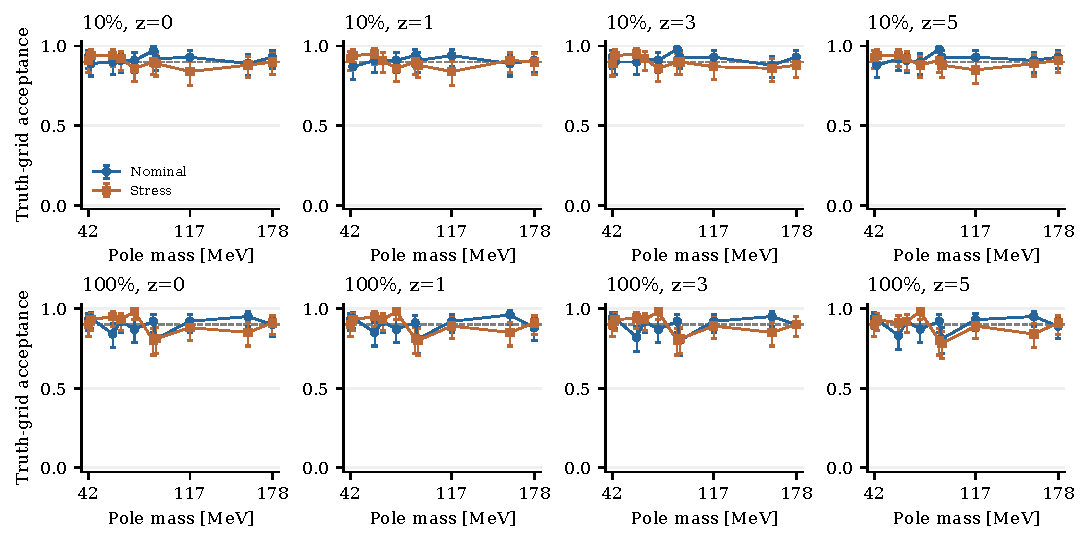
\includegraphics[width=\textwidth]{../figures/neyman_acceptance.pdf}\end{center}
{\small Held-out acceptance of the injected grid value using the frozen same-generator table; exact 95\% Clopper--Pearson intervals use each cell's valid independent evaluation denominator. The dashed line is 90\%. Intervals are pointwise; cells share backgrounds.\par}


For continuous $T$, the population lower-tail mass below the tenth calibration order statistic has the $\mathrm{Beta}(10,91)$ distribution. Its central 95\% reference interval implies acceptance between 83.6\% and 95.1\% before observing the calibration table. 

That order-statistic uncertainty is distinct from the held-out binomial interval and from the rank marginal size bound. It is not an extra confidence interval to add to a pull error.

At full-exposure 76 MeV, $z=5$, same-source frozen acceptance is nominal 87/100 (95\% CP [78.8\%, 92.9\%]) and stress 98/100 (95\% CP [93.0\%, 99.8\%]). These cells need not realize exactly 90\% acceptance.

The accepted set is retained as a discrete set. Its reported upper envelope is the largest accepted grid value; no interpolation or monotonic repair is applied. Empty sets, holes and acceptance of $z=8$ (right censoring) are explicit. An empty set is assigned the physical reporting convention $U=0$ and remains flagged; hence its upper bound contains $A=0$ even if the rank test rejects that grid point. Acceptance of the true grid point differs from containment by this upper envelope. The result supplies no off-grid coverage guarantee.

\clearpage\section*{Toy-CLs diagnostic and native profile limits}


The finite-grid toy diagnostic uses the same raw-yield ordering and distributions from a calibration cohort independent of evaluation:\[\CLs^{\rm toy}(A)=\min\{1,p_A(T)/p_0(T)\}.\]The same add-one rank probabilities are used in numerator and denominator. Reject at $\CLs^{\rm toy}\leq0.10$. Its rejection set is a subset of the rank-$p_A$ rejection set and inherits the conservative matched-generator marginal bound. With 100 calibration toys, this ratio has finite Monte Carlo resolution and substantial tail uncertainty; it is a diagnostic, not a high-precision CLs calibration. Its accepted grid and censoring records are preserved without interpolation.

\textbf{A finite-MC floor can hide failed transfer.} At 76 MeV, full-exposure stress $z=5$ toys with nominal calibration have 0/100 Neyman acceptance and 100 empty sets, yet toy CLs accepts 100/100 and has 100 right-censored endpoints. Here $p_A=p_0=1/101$ gives a ratio of one. This is finite-MC saturation, not successful calibration or a rescue of the native limit; native containment is also 0/100.

\begin{center}\footnotesize\begin{tabular}{lrrrrr}\toprule
Method & Source & Exposure & Accept $A$ & Envelope contains $A$ & Median endpoint/$s_0$\\\midrule
Neyman & Nominal & 10\% & 88--98 & 88--98 & 4.00--4.00\\
Neyman & Nominal & 100\% & 80--95 & 80--95 & 3.00--4.00\\
Neyman & Stress & 10\% & 86--95 & 86--95 & 4.00--4.00\\
Neyman & Stress & 100\% & 80--98 & 80--98 & 3.00--4.00\\
Toy CLs & Nominal & 10\% & 88--98 & 88--98 & 4.00--4.00\\
Toy CLs & Nominal & 100\% & 80--95 & 80--95 & 3.00--4.00\\
Toy CLs & Stress & 10\% & 87--96 & 87--96 & 4.00--4.00\\
Toy CLs & Stress & 100\% & 81--98 & 81--98 & 3.00--4.00\\
Native & Nominal & 100\% & 77--100 & 77--100 & 3.77--4.99\\
Native & Stress & 100\% & 0--100 & 0--100 & 0.20--16.77\\
\bottomrule\end{tabular}\end{center}


{\small At $z=3$: ranges across ten masses, with counts out of each cell's valid denominator (normally 100). Native acceptance and containment are the same upper-limit decision. A reported grid endpoint of 8 is a lower endpoint for a right-censored row, not a measured finite limit.\par}

\begin{center}\small\begin{tabular}{lrrrr}\toprule
$m$ [MeV] & Nominal $z=3$ & Nominal $z=5$ & Stress $z=3$ & Stress $z=5$\\\midrule
42 & 89/100 & 86/100 & 0/100 & 0/100\\
44 & 94/100 & 94/100 & 0/100 & 0/100\\
60 & 93/100 & 91/100 & 1/100 & 1/100\\
66 & 91/100 & 89/100 & 100/100 & 100/100\\
76 & 77/100 & 73/100 & 0/100 & 0/100\\
90 & 100/100 & 100/100 & 30/100 & 28/100\\
92 & 93/100 & 91/100 & 9/100 & 8/100\\
117 & 100/100 & 100/100 & 97/100 & 95/100\\
160 & 95/100 & 92/100 & 99/100 & 97/100\\
178 & 88/100 & 89/100 & 73/100 & 69/100\\
\bottomrule\end{tabular}\end{center}


{\small Full-exposure native 90\% profile-CLs upper-limit containment; each cell's exact 95\% Clopper--Pearson interval is supplied in \texttt{limit\_summary.csv}.\par}

The native calculation uses the original raw likelihood, with each toy's GP mean/covariance fixed during nuisance profiling. Its denominator is the free fit for $\Ah\geq0$ and the $A=0$ fit otherwise; the GP mean is the null Asimov spectrum. The inherited bounded-$\widetilde q$ asymptotic tails give the root $\CLs=0.10$. These full-exposure limits are never obtained by correcting a limit with $\widehat\delta$ or $\widehat R$. Toy-rank CLs and native profile CLs differ in ordering and approximation; agreement is an empirical result, not an identity.

\clearpage\section*{Accounting, source boundaries and reproducibility}


\textbf{Set accounting.} The following ranges are across all same-generator mass/strength cells. Counts record outcomes of 100 attempted evaluation toys per cell; they are not pooled rates. Complete per-cell valid counts, truth acceptance, upper-envelope containment, exact binomial intervals and set flags are retained.

\begin{center}\footnotesize\begin{tabular}{lrrrrrr}\toprule
Method & Source & Exposure & Valid & Empty & Holey & Right-censored\\\midrule
Neyman & Nominal & 10\% & 100--100 & 0--11 & 0--0 & 0--15\\
Neyman & Nominal & 100\% & 100--100 & 0--19 & 0--0 & 0--6\\
Neyman & Stress & 10\% & 100--100 & 0--16 & 0--0 & 0--12\\
Neyman & Stress & 100\% & 100--100 & 0--20 & 0--0 & 0--10\\
Toy CLs & Nominal & 10\% & 100--100 & 0--0 & 0--0 & 0--15\\
Toy CLs & Nominal & 100\% & 100--100 & 0--0 & 0--0 & 0--19\\
Toy CLs & Stress & 10\% & 100--100 & 0--0 & 0--0 & 0--16\\
Toy CLs & Stress & 100\% & 100--100 & 0--0 & 0--0 & 0--19\\
\bottomrule\end{tabular}\end{center}


\textbf{Generator provenance.} The nominal generator is the pinned 2016 GP arithmetic mean. The archived conditional stress histogram retains the failed broad-component source-fit flag in its source manifest. Neither is an independently validated physical-background model. Background-source estimation uncertainty is not sampled. The exact $0.1$ exposure branch here is not the historical 2016 subset: its archived support-count ratio is 0.1022, and exact luminosity fraction, selection equivalence and event overlap remain unverified.

\textbf{Fitting and failures.} The inherited signal resolution, pole-centered $\pm2.25\sigma_m$ masks and reviewed mass-dependent kernel parameters remain fixed. Each spectrum recomputes count-dependent log-GP targets/noise, arithmetic mean and correlated covariance; no hyperparameter optimization is performed. The signed-yield Poisson likelihood profiles the same correlated GP nuisance constraint. Numerical retries retain the original spectrum and toy ID. Validity gates concern finite objectives, gradients and positive Poisson means, not closeness to truth or nominal coverage. Unresolved rows remain in the failure ledger.

The historical 2016 support/optimizer-qualification exception remains. Successful fixed-kernel conditional toys do not validate the original kernel optimization or repair that source qualification.

\textbf{Frozen calibration uncertainty.} Offset, response and their covariance come from calibration toys only. Whole-toy resampling preserves null/injected partners, masses and nested exposure pairs. The primary held-out pull treats the table as fixed; the separate approximate delta-method error also uses $k_0$ and is labeled accordingly; it does not recalibrate a likelihood interval. The finite-rank guarantee assumes exchangeable calibration/evaluation at a fixed generator; it does not establish physical-source coverage.

\textbf{Reproduction.} The package saves the numerical protocol, pilot reference, independent cohorts, calibration table, per-toy rows, summary tables, failed-row ledger, source hashes, vector figures and this LaTeX source. \texttt{scripts/analyze.py} computes summaries; \texttt{scripts/make\_appendix.py --build} regenerates this appendix without fitting. The original 2021 PDF is copied and joined only during final packaging. \texttt{README.md} gives the validated commands. See the protocol and QA files for exact seeds, worker limits, completeness and final validation status.

The master seed is \texttt{63420160924}; uncertainty summaries use 2,000 whole-toy bootstrap replicates. Calibration and evaluation bootstrap streams are separate. The deterministic mean-spectrum fits in \texttt{asimov\_rows.csv} are not additional toys.

\textbf{Claim boundary.} This study can measure conditional offset scaling, response transfer and finite-toy performance under two pinned generators. It cannot establish unconditional coverage over unknown backgrounds, physical-model adequacy, calibrated discovery/global significance or an experimental exclusion.

\textbf{Reference.} Particle Data Group, \emph{Statistics} (2026), sections 40.2 and 40.4.2, \url{https://pdg.lbl.gov/2026/reviews/rpp2026-rev-statistics.pdf}. General bias and Neyman-construction context; the exposure approximation and finite-rank convention are defined explicitly above.

\end{document}